\subsection{Design und Planung}
Die Konstruktion unseres Miniatur-Cybertrucks war durch das ikonische Design des Tesla Cybertrucks inspiriert. Unser Modell wurde im Maßstab 1:17 entworfen, um eine hohe Authentizität zu gewährleisten. Die Planung und das Design erfolgten in Autodesk Inventor, einer fortgeschrittenen CAD-Software, die vor allem auf professionelle Nutzer abzielt. Trotz der anfänglichen Herausforderungen aufgrund der Komplexität der Software, erwies sich die Entscheidung als richtig, da sie es ermöglichte, präzise und detaillierte Modelle zu erstellen, die den Anforderungen unseres Projekts gerecht wurden.

\newpage

\subsection{Anpassung des Chassis}
Das Chassis wurde speziell entworfen, um Komponenten wie Raspberry Pi, ein Breadboard, Motoren, Batterien und Sensoren aufzunehmen. Eine besondere Herausforderung stellte die Platzierung der Ultraschallsensoren dar, da der begrenzte Raum eine optimale Anordnung erschwerte. Durch den Einsatz von Autodesk Inventor konnten wir die Sensoren virtuell positionieren und ihre Ausrichtung so anpassen, dass sie funktional innerhalb des begrenzten Raums operieren konnten.

\subsection{3D-Druck und Komponentenintegration}
Das Chassis wurde extern mittels 3D-Druck in PLA gefertigt, was uns erlaubte, eine präzise und robuste Struktur zu schaffen. Die vorhandenen 3D-Modelle der elektronischen Komponenten wie des Raspberry Pi wurden direkt in das CAD-Modell integriert, was die Konstruktion erheblich vereinfachte. Die Modulbauweise in Autodesk Inventor ermöglichte es uns, das Projekt als Baugruppe zu verwalten, wodurch der gesamte Designprozess modularer und flexibler wurde.

\subsection{Entwicklung des Greifarms}
Der Greifarm, ein zentraler Bestandteil unseres selbstfahrenden Golfcars, wurde entworfen, um Golfbälle aufzunehmen und zu transportieren. Die Konstruktion dieses Mechanismus nutzte einen SG90 Servomotor, der für seine Zuverlässigkeit und Effizienz in Leichtbauanwendungen bekannt ist.

\subsubsection{Konstruktionsprozess}
Die Entwicklung des Greifarms war durch einen iterativen Ansatz geprägt, bei dem mehrere Prototypen in verschiedenen Größen gedruckt wurden, um die optimale Passform für den Golfball zu ermitteln. Dieser Prozess ermöglichte es uns, präzise Anpassungen an den Dimensionen und der Funktionalität des Greifarms vorzunehmen, um eine maximale Effizienz und Zuverlässigkeit zu gewährleisten.

\subsubsection{Material und Montage}
Obwohl die Konstruktion des Greifarms relativ einfach war, erforderte sie präzise Fertigungstechniken, um die gewünschten Ergebnisse zu erzielen. Nachdem die endgültige Version des Greifarms durch 3D-Druck hergestellt wurde, entschieden wir uns für eine einfache, jedoch effektive Befestigungsmethode: Der Arm wurde mit Heißkleber an der Vorderseite des Fahrzeugs fixiert. Trotz der möglicherweise fragwürdigen Wahl dieses Befestigungsmittels erfüllte diese Lösung ihren Zweck ohne Probleme und bestätigte die Funktionalität des Greifarms unter realen Bedingungen.

\begin{figure}[H]
\centering
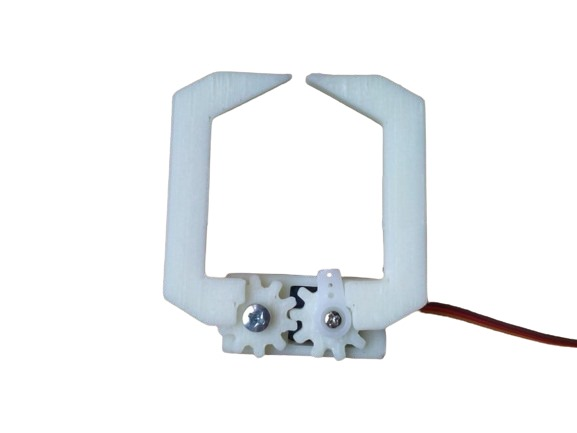
\includegraphics[width=1\textwidth]{Resources/claw_gripper.jpg}
\caption{Der entwickelte Greifarm mit SG90 Servomotor.}
\end{figure}

\subsubsection{Ergebnis und Bewertung}
Die Verwendung des SG90 Servomotors erwies sich als eine ausgezeichnete Wahl für die Steuerung des Greifarms, da er genügend Drehmoment für die Handhabung der Golfbälle bietet, ohne das Gesamtgewicht des Fahrzeugs wesentlich zu erhöhen. Die endgültige Montage, obwohl einfach durchgeführt, zeigte eine robuste Leistung während aller Testphasen und im realen Einsatz auf dem "Spielfeld".

\subsection{Problematische Kameraplatzierung}
Ein spezifisches Problem war die Platzierung der Kamera, die wir als "Kameranase" des Fahrzeugs bezeichnen. Die einzige praktikable Lösung, die sich im Rahmen des Designs anbieten ließ, war nicht optimal, da sie Kompromisse in Bezug auf die Sicht und die Ästhetik erforderte. Dennoch war diese Anordnung notwendig, um die Funktionalität des Fahrzeugs in einem realen Umfeld sicherzustellen.

\subsection{Bilder der Konstruktion}
Um einen detaillierten Einblick in die Konstruktionsphase zu geben, zeigen wir hier einige Bilder des Modells aus verschiedenen Perspektiven:

\newpage

\begin{figure}[h]
    \centering
    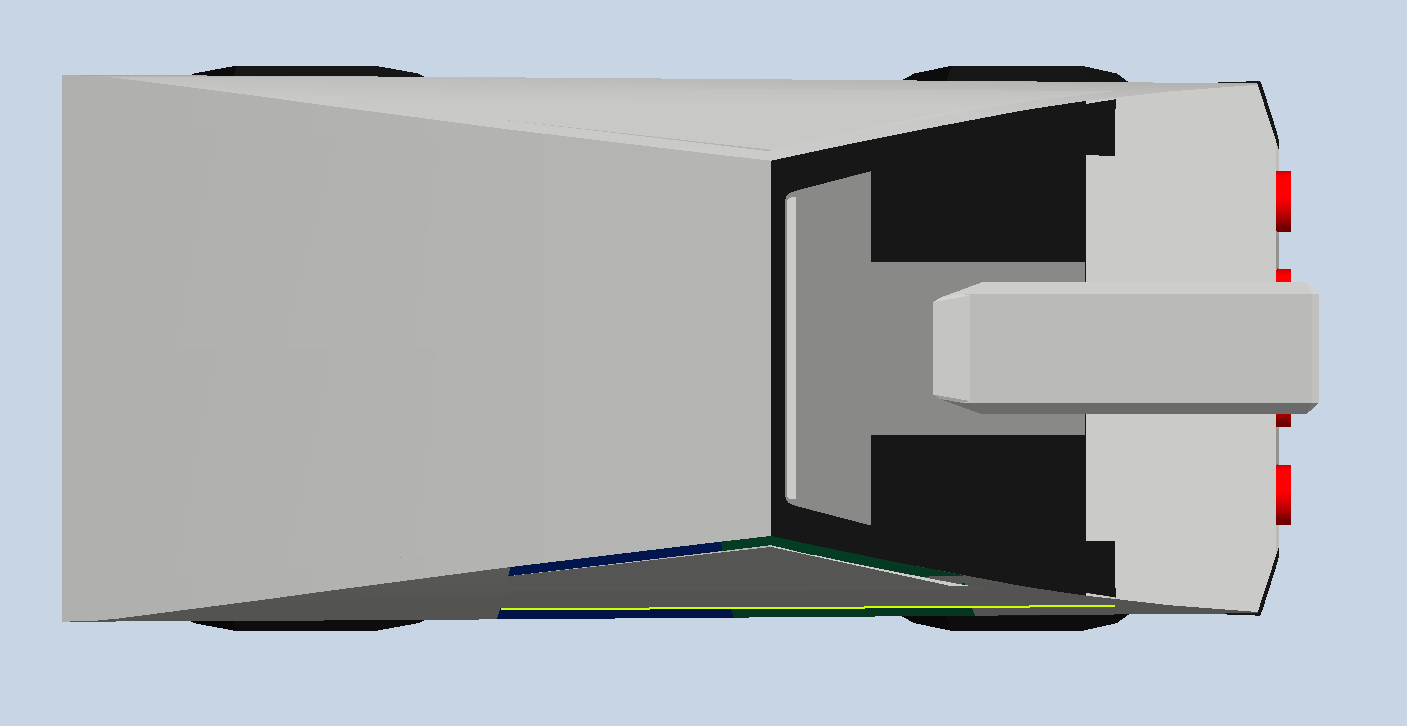
\includegraphics[width=0.95\textwidth]{Resources/oben_normal.png}
    \caption{Ansicht von oben (normal)}
\end{figure}

\begin{figure}[h]
    \centering
    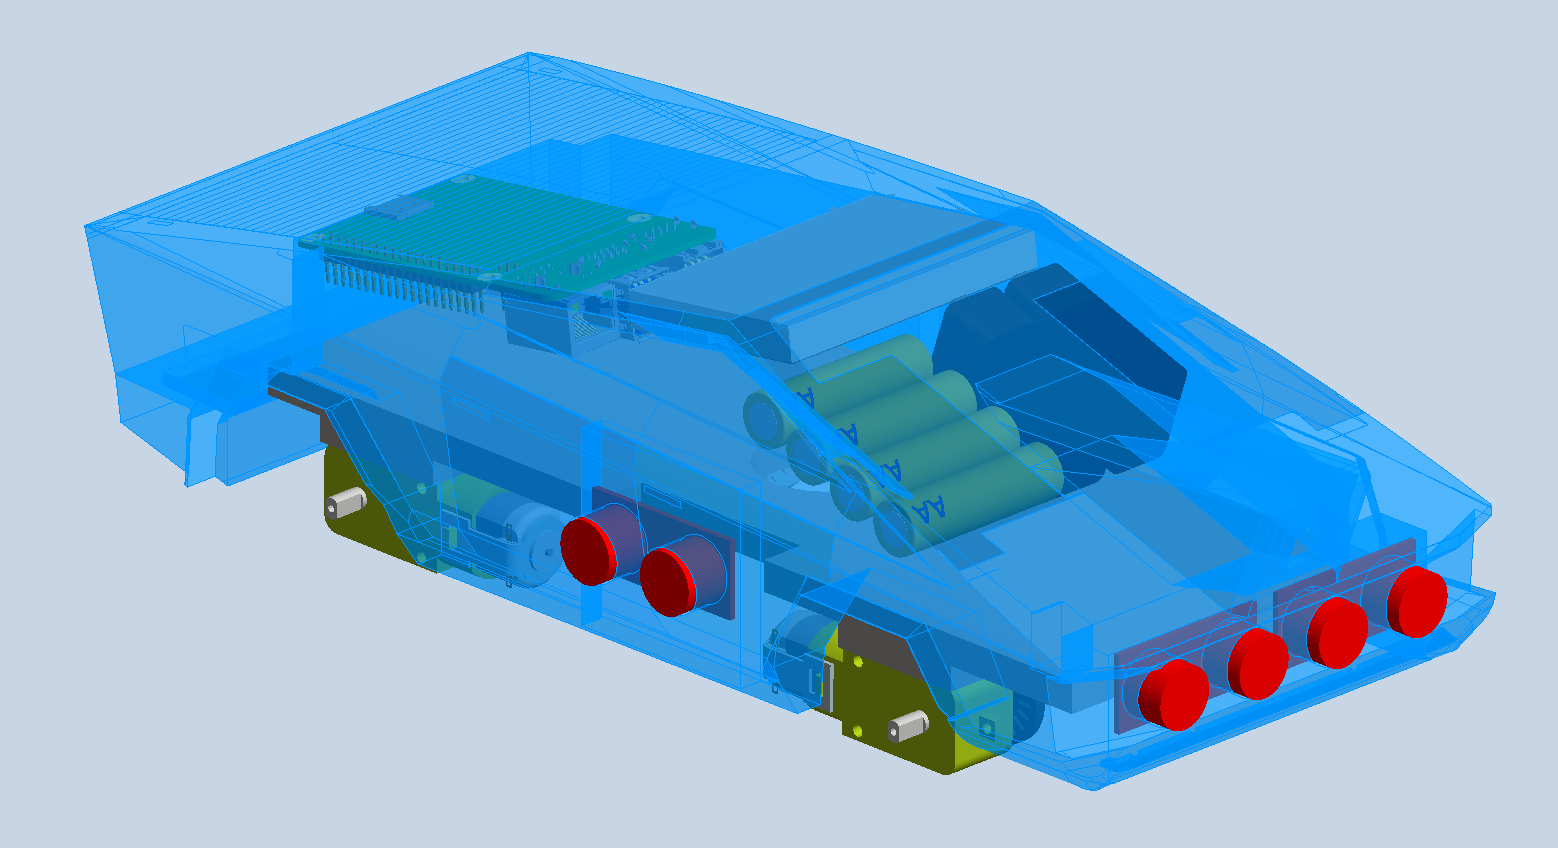
\includegraphics[width=0.95\textwidth]{Resources/seitlich_chassi_transparent.png}
    \caption{Seitenansicht des Chassis (transparent)}
\end{figure}

\newpage

\begin{figure}[h]
    \centering
    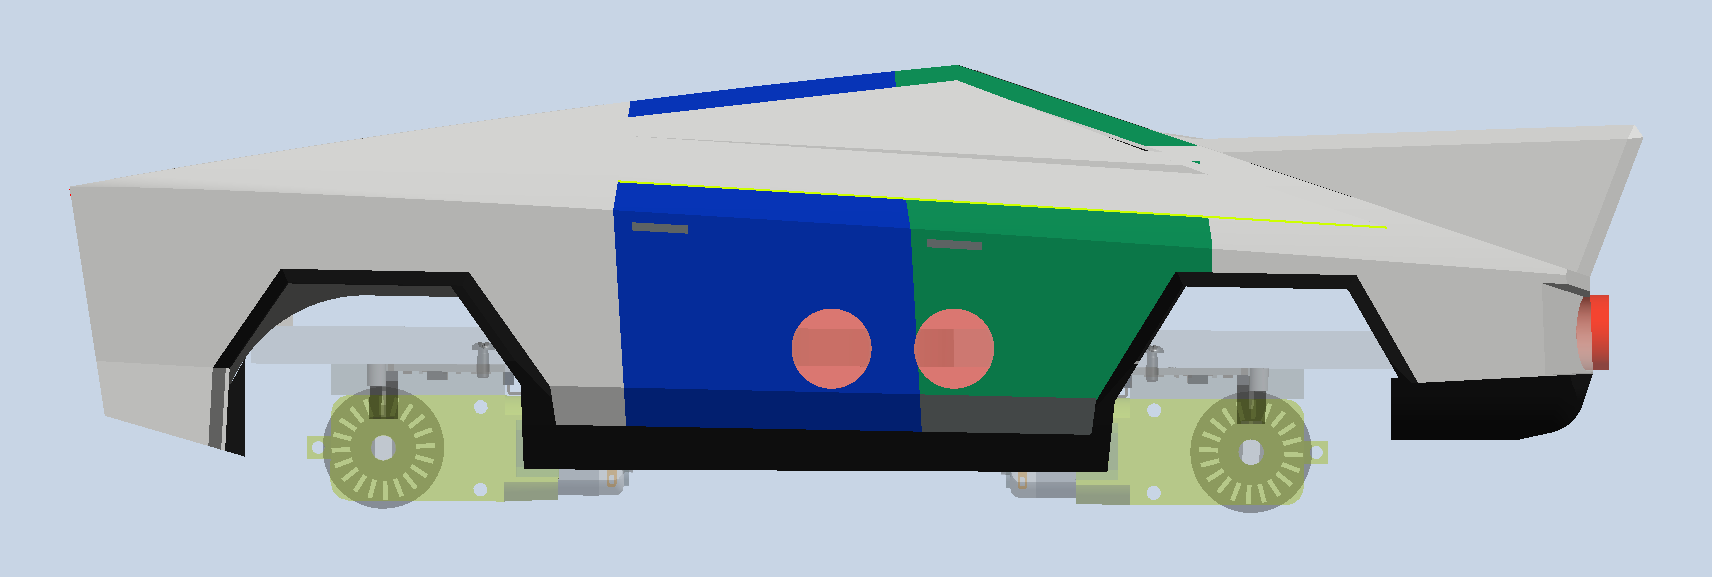
\includegraphics[width=0.99\textwidth]{Resources/seitlich_transparent.png}
    \caption{Seitenansicht (transparent)}
\end{figure}

\begin{figure}[h]
    \centering
    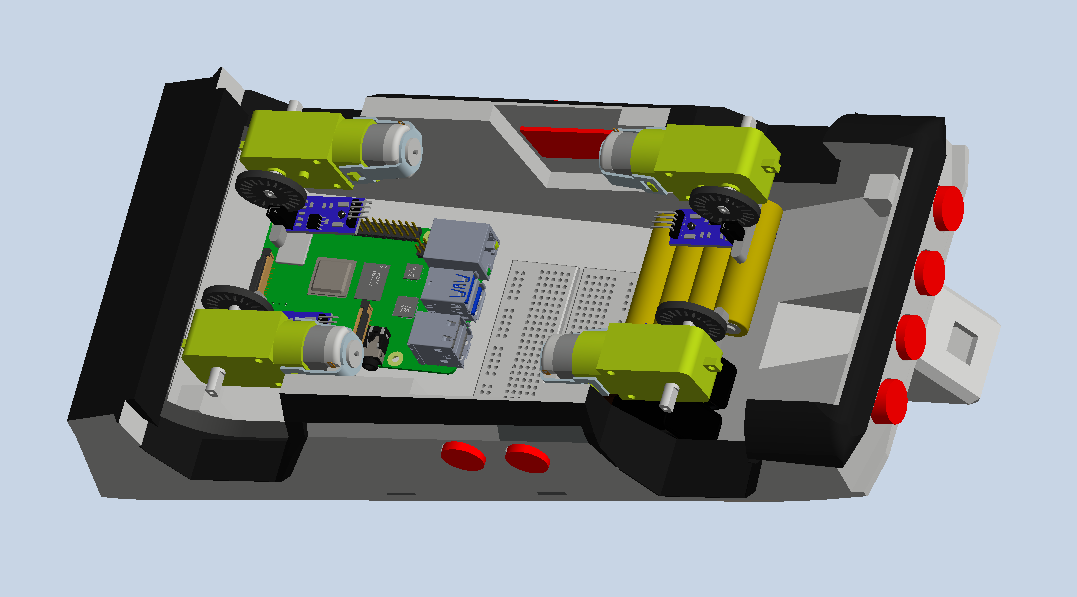
\includegraphics[width=0.99\textwidth]{Resources/unten_ohne_trennplatte.png}
    \caption{Ansicht von unten ohne Trennplatte}
\end{figure}

\newpage

\begin{figure}[h]
    \centering
    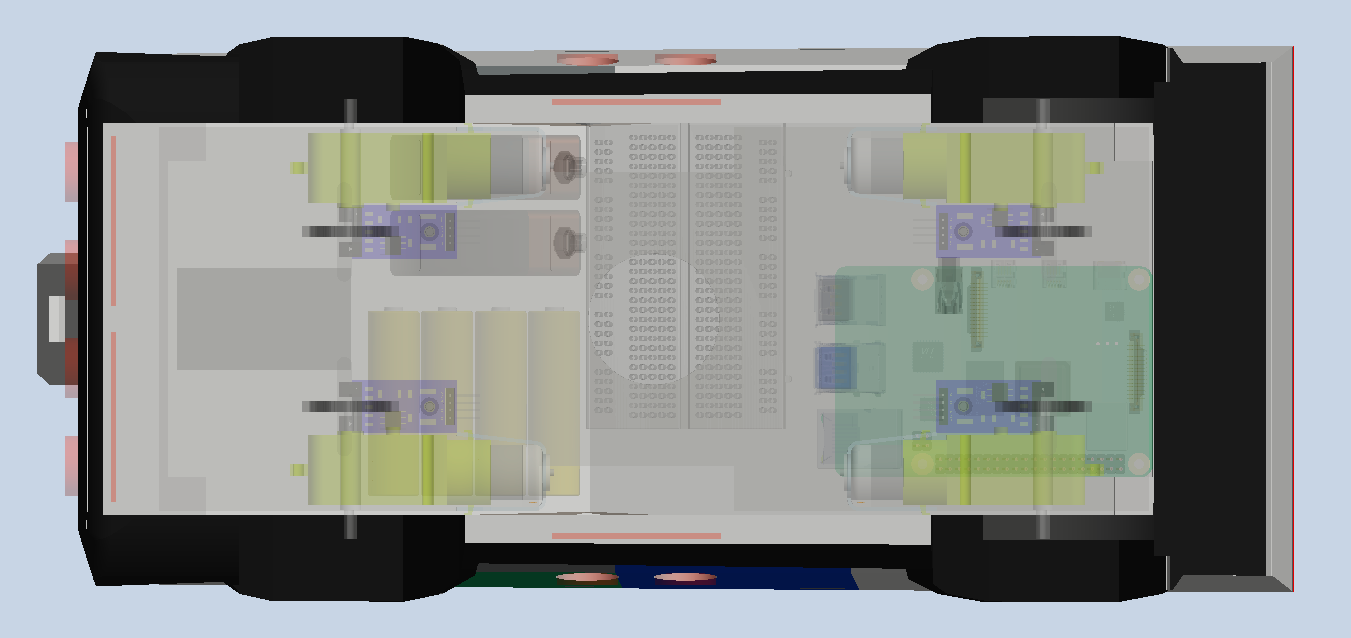
\includegraphics[width=0.95\textwidth]{Resources/unten_transparent.png}
    \caption{Unteransicht (transparent)}
\end{figure}

\begin{figure}[h]
    \centering
    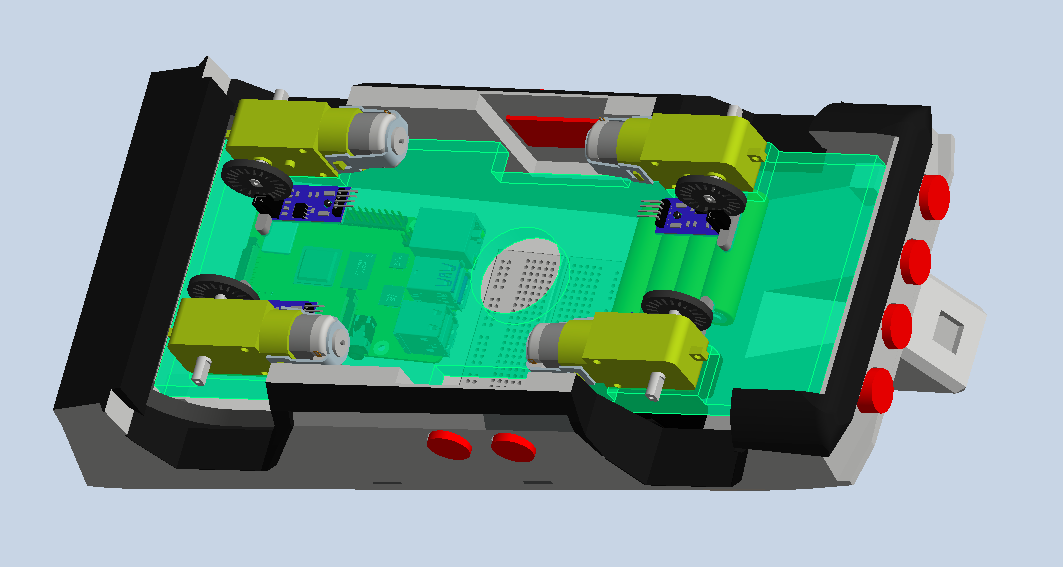
\includegraphics[width=0.95\textwidth]{Resources/unten_trennplatte_transparent.png}
    \caption{Unteransicht mit Trennplatte (transparent)}
\end{figure}

\newpage

\subsubsection{3D-Modellansicht Online}
Um eine interaktive Betrachtung unseres Konstruktionsmodells zu ermöglichen, stellen wir das 3D-Modell über den Autodesk Viewer online zur Verfügung. Dieser Service erlaubt es Nutzern, das Modell in hoher Detailgenauigkeit zu betrachten, ohne spezielle Software installieren zu müssen.

\paragraph{Funktionen des Autodesk Viewers}
Über den folgenden Link kann das 3D-Modell unseres Miniatur-Cybertrucks in Echtzeit betrachtet werden: \newline \url{https://tinyurl.com/golfcarspace}.
\newline
Mit diesem Tool können Nutzer:

\begin{itemize}
    \item Das Modell aus verschiedenen Winkeln betrachten und um 360 Grad drehen.
    \item In bestimmte Bereiche hinein- und herauszoomen, um spezifische Details zu erkunden.
    \item Verschiedene Ansichten aktivieren, wie transparente Ansichten, um einen Einblick in die interne Platzierung der Komponenten zu erhalten.
    \item Schnittebenen hinzufügen, um Querschnitte des Modells zu analysieren und zu verstehen, wie die einzelnen Teile zusammenpassen.
\end{itemize}

Diese Online-Plattform bietet eine wertvolle Ressource für Kunden und Interessenten, um die technischen Aspekte und die konzeptionelle Gestaltung unseres Projekts tiefgehend zu verstehen. Sie dient nicht nur der Darstellung unseres technologischen Know-hows, sondern ermöglicht auch eine transparente Kommunikation der konstruktiven Leistungen unseres Teams.


\subsection{Schlussfolgerung}
Die Konstruktion unseres Miniatur-Cybertrucks war ein umfangreiches Projekt, das präzise Planung, sorgfältige Ausführung und kreatives Problemlösen erforderte. Die erfolgreiche Umsetzung dieses Teils des Projekts demonstriert unsere Fähigkeit, komplexe technische Herausforderungen zu meistern und innovative Lösungen zu entwickeln.

\newpage
